% Options for packages loaded elsewhere
\PassOptionsToPackage{unicode}{hyperref}
\PassOptionsToPackage{hyphens}{url}
\PassOptionsToPackage{dvipsnames,svgnames,x11names}{xcolor}
\documentclass[
  10pt,
]{report}
\usepackage{xcolor}
\usepackage[margin=0.85in]{geometry}
\usepackage{amsmath,amssymb}
\setcounter{secnumdepth}{5}
\usepackage{iftex}
\ifPDFTeX
  \usepackage[T1]{fontenc}
  \usepackage[utf8]{inputenc}
  \usepackage{textcomp} % provide euro and other symbols
\else % if luatex or xetex
  \usepackage{unicode-math} % this also loads fontspec
  \defaultfontfeatures{Scale=MatchLowercase}
  \defaultfontfeatures[\rmfamily]{Ligatures=TeX,Scale=1}
\fi
\usepackage{lmodern}
\ifPDFTeX\else
  % xetex/luatex font selection
\fi
% Use upquote if available, for straight quotes in verbatim environments
\IfFileExists{upquote.sty}{\usepackage{upquote}}{}
\IfFileExists{microtype.sty}{% use microtype if available
  \usepackage[]{microtype}
  \UseMicrotypeSet[protrusion]{basicmath} % disable protrusion for tt fonts
}{}
\makeatletter
\@ifundefined{KOMAClassName}{% if non-KOMA class
  \IfFileExists{parskip.sty}{%
    \usepackage{parskip}
  }{% else
    \setlength{\parindent}{0pt}
    \setlength{\parskip}{6pt plus 2pt minus 1pt}}
}{% if KOMA class
  \KOMAoptions{parskip=half}}
\makeatother
\usepackage{color}
\usepackage{fancyvrb}
\newcommand{\VerbBar}{|}
\newcommand{\VERB}{\Verb[commandchars=\\\{\}]}
\DefineVerbatimEnvironment{Highlighting}{Verbatim}{commandchars=\\\{\}}
% Add ',fontsize=\small' for more characters per line
\newenvironment{Shaded}{}{}
\newcommand{\AlertTok}[1]{\textcolor[rgb]{1.00,0.00,0.00}{\textbf{#1}}}
\newcommand{\AnnotationTok}[1]{\textcolor[rgb]{0.38,0.63,0.69}{\textbf{\textit{#1}}}}
\newcommand{\AttributeTok}[1]{\textcolor[rgb]{0.49,0.56,0.16}{#1}}
\newcommand{\BaseNTok}[1]{\textcolor[rgb]{0.25,0.63,0.44}{#1}}
\newcommand{\BuiltInTok}[1]{\textcolor[rgb]{0.00,0.50,0.00}{#1}}
\newcommand{\CharTok}[1]{\textcolor[rgb]{0.25,0.44,0.63}{#1}}
\newcommand{\CommentTok}[1]{\textcolor[rgb]{0.38,0.63,0.69}{\textit{#1}}}
\newcommand{\CommentVarTok}[1]{\textcolor[rgb]{0.38,0.63,0.69}{\textbf{\textit{#1}}}}
\newcommand{\ConstantTok}[1]{\textcolor[rgb]{0.53,0.00,0.00}{#1}}
\newcommand{\ControlFlowTok}[1]{\textcolor[rgb]{0.00,0.44,0.13}{\textbf{#1}}}
\newcommand{\DataTypeTok}[1]{\textcolor[rgb]{0.56,0.13,0.00}{#1}}
\newcommand{\DecValTok}[1]{\textcolor[rgb]{0.25,0.63,0.44}{#1}}
\newcommand{\DocumentationTok}[1]{\textcolor[rgb]{0.73,0.13,0.13}{\textit{#1}}}
\newcommand{\ErrorTok}[1]{\textcolor[rgb]{1.00,0.00,0.00}{\textbf{#1}}}
\newcommand{\ExtensionTok}[1]{#1}
\newcommand{\FloatTok}[1]{\textcolor[rgb]{0.25,0.63,0.44}{#1}}
\newcommand{\FunctionTok}[1]{\textcolor[rgb]{0.02,0.16,0.49}{#1}}
\newcommand{\ImportTok}[1]{\textcolor[rgb]{0.00,0.50,0.00}{\textbf{#1}}}
\newcommand{\InformationTok}[1]{\textcolor[rgb]{0.38,0.63,0.69}{\textbf{\textit{#1}}}}
\newcommand{\KeywordTok}[1]{\textcolor[rgb]{0.00,0.44,0.13}{\textbf{#1}}}
\newcommand{\NormalTok}[1]{#1}
\newcommand{\OperatorTok}[1]{\textcolor[rgb]{0.40,0.40,0.40}{#1}}
\newcommand{\OtherTok}[1]{\textcolor[rgb]{0.00,0.44,0.13}{#1}}
\newcommand{\PreprocessorTok}[1]{\textcolor[rgb]{0.74,0.48,0.00}{#1}}
\newcommand{\RegionMarkerTok}[1]{#1}
\newcommand{\SpecialCharTok}[1]{\textcolor[rgb]{0.25,0.44,0.63}{#1}}
\newcommand{\SpecialStringTok}[1]{\textcolor[rgb]{0.73,0.40,0.53}{#1}}
\newcommand{\StringTok}[1]{\textcolor[rgb]{0.25,0.44,0.63}{#1}}
\newcommand{\VariableTok}[1]{\textcolor[rgb]{0.10,0.09,0.49}{#1}}
\newcommand{\VerbatimStringTok}[1]{\textcolor[rgb]{0.25,0.44,0.63}{#1}}
\newcommand{\WarningTok}[1]{\textcolor[rgb]{0.38,0.63,0.69}{\textbf{\textit{#1}}}}
\usepackage{longtable,booktabs,array}
\usepackage{calc} % for calculating minipage widths
% Correct order of tables after \paragraph or \subparagraph
\usepackage{etoolbox}
\makeatletter
\patchcmd\longtable{\par}{\if@noskipsec\mbox{}\fi\par}{}{}
\makeatother
% Allow footnotes in longtable head/foot
\IfFileExists{footnotehyper.sty}{\usepackage{footnotehyper}}{\usepackage{footnote}}
\makesavenoteenv{longtable}
\setlength{\emergencystretch}{3em} % prevent overfull lines
\providecommand{\tightlist}{%
  \setlength{\itemsep}{0pt}\setlength{\parskip}{0pt}}
\usepackage{tikz}
\usetikzlibrary{arrows.meta,positioning,shapes.geometric,shapes.misc,fit}
\usepackage{bookmark}
\IfFileExists{xurl.sty}{\usepackage{xurl}}{} % add URL line breaks if available
\urlstyle{same}
\hypersetup{
  pdftitle={Building Durable Workflows in EDSL},
  pdfauthor={Expected Parrot},
  colorlinks=true,
  linkcolor={blue},
  filecolor={Maroon},
  citecolor={Blue},
  urlcolor={blue},
  pdfcreator={LaTeX via pandoc}}

\title{Building Durable Workflows in EDSL}
\usepackage{etoolbox}
\makeatletter
\providecommand{\subtitle}[1]{% add subtitle to \maketitle
  \apptocmd{\@title}{\par {\large #1 \par}}{}{}
}
\makeatother
\subtitle{Dependencies, human delivery, simulated respondents, derived
values, repetition, and recovery}
\author{Expected Parrot}
\date{September 2026}

\begin{document}
\maketitle

{
\hypersetup{linkcolor=}
\setcounter{tocdepth}{3}
\tableofcontents
}
\chapter{Purpose and scope}\label{purpose-and-scope}

An EDSL workflow coordinates work performed by people, language-model
agents, or a mixture of both. It decides who receives each task, when a
task becomes available, which earlier answers it may observe, how
results are combined, and what happens after failures or restarts.

The workflow layer is deliberately separate from delivery. Humanize can
create private surveys, send invitations, and collect responses. A
simulated inbox can deliver the same work to EDSL agents. The workflow
coordinator remains the authority that decides what becomes ready next.

This manual describes the implementation in \texttt{edsl.workflows}. It
covers:

\begin{itemize}
\tightlist
\item
  dependency graphs and work-item lifecycles;
\item
  participant selection, fan-out, and fan-in;
\item
  typed answer, output, and submission references;
\item
  serializable conditions and deterministic derived values;
\item
  bounded repeat blocks;
\item
  visibility and anonymity boundaries;
\item
  shared-state reads and writes;
\item
  human delivery and LLM simulation;
\item
  durable retries, leases, and process recovery;
\item
  SQLite persistence and DAG visualization; and
\item
  reusable design patterns and current limitations.
\end{itemize}

The workflow API is experimental. The serialized form and behavior
described here are the current implementation, not a promise of
permanent compatibility.

\chapter{The central idea}\label{the-central-idea}

A workflow turns a declarative graph into durable, respondent-specific
work:

\begin{figure}[htbp]
\centering
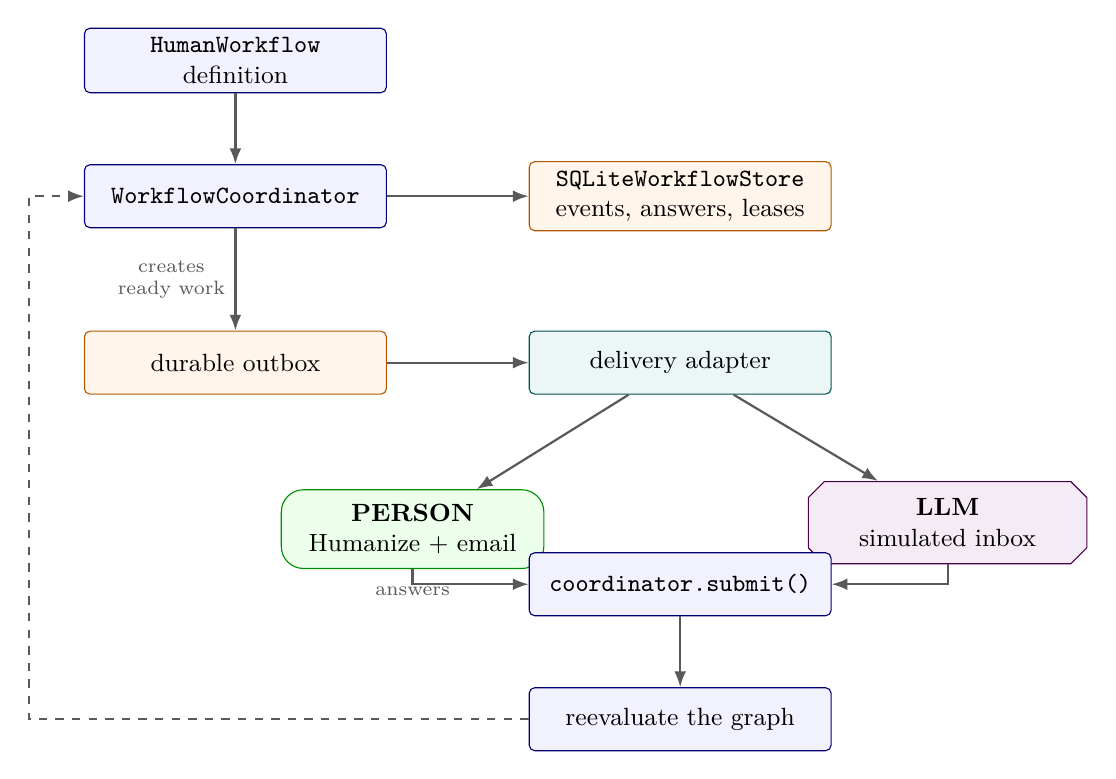
\begin{tikzpicture}[
  font=\small,
  box/.style={draw=blue!45!black, rounded corners=2pt, fill=blue!5,
    align=center, minimum height=8mm, text width=36mm},
  store/.style={box, draw=orange!70!black, fill=orange!8},
  delivery/.style={box, draw=teal!65!black, fill=teal!7},
  human/.style={draw=green!55!black, rounded corners=8pt, fill=green!8,
    align=center, minimum height=10mm, text width=31mm},
  llm/.style={draw=violet!60!black, chamfered rectangle, chamfered rectangle corners=all,
    fill=violet!8, align=center, minimum height=10mm, text width=31mm},
  flow/.style={-{Latex[length=2mm]}, thick, draw=black!65},
  note/.style={font=\scriptsize, text=black!65, align=center}
]
\node[box] (definition) {\texttt{HumanWorkflow}\\definition};
\node[box, below=9mm of definition] (coordinator) {\texttt{WorkflowCoordinator}};
\node[store, right=18mm of coordinator] (store) {\texttt{SQLiteWorkflowStore}\\events, answers, leases};
\node[store, below=13mm of coordinator] (outbox) {durable outbox};
\node[delivery, right=18mm of outbox] (adapter) {delivery adapter};
\node[human, below left=12mm and -2mm of adapter] (humanize)
  {\textbf{PERSON}\\Humanize + email};
\node[llm, below right=12mm and -2mm of adapter] (simulated)
  {\textbf{LLM}\\simulated inbox};
\node[box, below=20mm of adapter] (submit) {\texttt{coordinator.submit()}};
\node[box, below=9mm of submit] (evaluate) {reevaluate the graph};

\draw[flow] (definition) -- (coordinator);
\draw[flow] (coordinator) -- (store);
\draw[flow] (coordinator) -- node[note, left]{creates\\ready work} (outbox);
\draw[flow] (outbox) -- (adapter);
\draw[flow] (adapter) -- (humanize);
\draw[flow] (adapter) -- (simulated);
\draw[flow] (humanize) |- node[note, below, pos=.25]{answers} (submit);
\draw[flow] (simulated) |- (submit);
\draw[flow] (submit) -- (evaluate);
\draw[flow, dashed] (evaluate.west) -| ([xshift=-7mm]coordinator.west) -- (coordinator.west);
\end{tikzpicture}
\caption{A workflow definition is evaluated by the coordinator, persisted in the
store, and delivered through interchangeable human or LLM channels. Green
rounded actors are people; violet clipped-corner actors are LLMs.}
\label{fig:workflow-architecture}
\end{figure}

The key invariant is:

\begin{quote}
Delivery systems do not decide workflow order. They deliver ready work
and return answers. Only the coordinator evaluates dependencies and
conditions.
\end{quote}

This separation allows the same definition to run with real respondents
during fieldwork and with LLM respondents during design, testing, and
stress analysis.

\section{Who performs the work?}\label{who-performs-the-work}

The workflow definition says who is eligible for a step by selecting a
participant role. It does \textbf{not} currently say whether that
participant is a person or an LLM. That choice belongs to execution:

\begin{longtable}[]{@{}
  >{\raggedright\arraybackslash}p{(\linewidth - 4\tabcolsep) * \real{0.3333}}
  >{\raggedright\arraybackslash}p{(\linewidth - 4\tabcolsep) * \real{0.3333}}
  >{\raggedright\arraybackslash}p{(\linewidth - 4\tabcolsep) * \real{0.3333}}@{}}
\toprule\noalign{}
\begin{minipage}[b]{\linewidth}\raggedright
Execution path
\end{minipage} & \begin{minipage}[b]{\linewidth}\raggedright
Performer
\end{minipage} & \begin{minipage}[b]{\linewidth}\raggedright
Mechanism
\end{minipage} \\
\midrule\noalign{}
\endhead
\bottomrule\noalign{}
\endlastfoot
Human fieldwork & \textbf{PERSON} & A Humanize delivery adapter emails a
private survey and imports the response. \\
Simulation & \textbf{LLM} & \texttt{WorkflowSimulation} opens ready
items and an \texttt{EDSLAgentAnswerer} runs their surveys with a
model. \\
Deterministic test & \textbf{SCRIPT} & A scripted answerer supplies
known responses without a person or model. \\
\end{longtable}

This neutrality is useful: one serialized protocol can be rehearsed with
LLMs and later deployed unchanged to people. It also means that diagrams
in this manual mark the \textbf{execution path}, not a property embedded
in \texttt{HumanStep}. Green rounded actor nodes mean a person; violet
clipped-corner actor nodes mean an LLM.

Performer routing is declared separately from the scientific workflow:

\begin{Shaded}
\begin{Highlighting}[]
\ImportTok{from}\NormalTok{ edsl.workflows }\ImportTok{import}\NormalTok{ ExecutionPlan, human, llm, role}

\NormalTok{plan }\OperatorTok{=}\NormalTok{ (}
\NormalTok{    ExecutionPlan()}
\NormalTok{    .bind(role(}\StringTok{"field{-}researcher"}\NormalTok{), human(channel}\OperatorTok{=}\StringTok{"humanize{-}email"}\NormalTok{))}
\NormalTok{    .bind(role(}\StringTok{"coder"}\NormalTok{), llm(model\_policy}\OperatorTok{=}\StringTok{"research{-}coder"}\NormalTok{))}
\NormalTok{)}
\end{Highlighting}
\end{Shaded}

The plan round-trips through \texttt{to\_dict()} and
\texttt{from\_dict()}, requires exactly one matching binding per
participant, and lets \texttt{WorkflowSimulation} select distinct
answerers by executor kind. Production still needs an adapter registry
that dispatches the human bindings to Humanize and persists the resolved
executor on each attempt. Step metadata may describe the intended
performer for diagrams, but it is not the routing authority.

\section{Waiting for optional work}\label{waiting-for-optional-work}

Normal \texttt{after=} dependencies propagate a predecessor's skip. Use
\texttt{after\_settled=} when a downstream step must wait for optional
work but should still run if that work is skipped:

\begin{Shaded}
\begin{Highlighting}[]
\NormalTok{builder.step(}
    \StringTok{"draft{-}report"}\NormalTok{,}
\NormalTok{    report\_survey,}
\NormalTok{    assigned\_to}\OperatorTok{=}\NormalTok{role(}\StringTok{"report{-}writer"}\NormalTok{),}
\NormalTok{    after\_settled}\OperatorTok{=}\NormalTok{human\_adjudication,}
\NormalTok{)}
\end{Highlighting}
\end{Shaded}

Both dependency modes wait until every predecessor item is completed or
skipped. Only \texttt{after=} treats a skipped predecessor as a reason
to skip the consumer.

\chapter{A first workflow}\label{a-first-workflow}

Suppose one person proposes a weekend activity and a second person
approves it.

\begin{Shaded}
\begin{Highlighting}[]
\ImportTok{from}\NormalTok{ edsl }\ImportTok{import}\NormalTok{ Agent, QuestionFreeText, QuestionYesNo, Survey}
\ImportTok{from}\NormalTok{ edsl.workflows }\ImportTok{import}\NormalTok{ Workflow, role}

\NormalTok{builder }\OperatorTok{=}\NormalTok{ Workflow(}\StringTok{"Weekend activity approval"}\NormalTok{)}

\NormalTok{activity }\OperatorTok{=}\NormalTok{ QuestionFreeText(}
\NormalTok{    question\_name}\OperatorTok{=}\StringTok{"activity"}\NormalTok{,}
\NormalTok{    question\_text}\OperatorTok{=}\StringTok{"Suggest a weekend activity."}\NormalTok{,}
\NormalTok{)}
\NormalTok{proposal }\OperatorTok{=}\NormalTok{ builder.step(}
    \StringTok{"propose"}\NormalTok{,}
\NormalTok{    Survey([activity]),}
\NormalTok{    assigned\_to}\OperatorTok{=}\NormalTok{role(}\StringTok{"proposer"}\NormalTok{),}
\NormalTok{)}

\NormalTok{approved }\OperatorTok{=}\NormalTok{ QuestionYesNo(}
\NormalTok{    question\_name}\OperatorTok{=}\StringTok{"approved"}\NormalTok{,}
\NormalTok{    question\_text}\OperatorTok{=}\NormalTok{(}
        \StringTok{"The proposed activity is "}
        \SpecialStringTok{f"}\SpecialCharTok{\{}\NormalTok{proposal}\SpecialCharTok{.}\NormalTok{answer(activity)}\SpecialCharTok{.}\NormalTok{template}\SpecialCharTok{\}}\SpecialStringTok{. Do you approve?"}
\NormalTok{    ),}
\NormalTok{)}
\NormalTok{builder.step(}
    \StringTok{"approve"}\NormalTok{,}
\NormalTok{    Survey([approved]),}
\NormalTok{    assigned\_to}\OperatorTok{=}\NormalTok{role(}\StringTok{"approver"}\NormalTok{),}
\NormalTok{    after}\OperatorTok{=}\NormalTok{proposal,}
\NormalTok{)}

\NormalTok{workflow }\OperatorTok{=}\NormalTok{ builder.}\BuiltInTok{compile}\NormalTok{()}
\end{Highlighting}
\end{Shaded}

The second task is not merely listed after the first in Python. Its
serialized definition contains an explicit dependency on
\texttt{propose}. The question also contains a typed reference to the
proposal answer.

Participants are ordinary EDSL agents whose traits determine their
roles:

\begin{Shaded}
\begin{Highlighting}[]
\NormalTok{participants }\OperatorTok{=}\NormalTok{ [}
\NormalTok{    Agent(}
\NormalTok{        name}\OperatorTok{=}\StringTok{"proposer@example.com"}\NormalTok{,}
\NormalTok{        traits}\OperatorTok{=}\NormalTok{\{}\StringTok{"role"}\NormalTok{: }\StringTok{"proposer"}\NormalTok{, }\StringTok{"email"}\NormalTok{: }\StringTok{"proposer@example.com"}\NormalTok{\},}
\NormalTok{    ),}
\NormalTok{    Agent(}
\NormalTok{        name}\OperatorTok{=}\StringTok{"approver@example.com"}\NormalTok{,}
\NormalTok{        traits}\OperatorTok{=}\NormalTok{\{}\StringTok{"role"}\NormalTok{: }\StringTok{"approver"}\NormalTok{, }\StringTok{"email"}\NormalTok{: }\StringTok{"approver@example.com"}\NormalTok{\},}
\NormalTok{    ),}
\NormalTok{]}
\end{Highlighting}
\end{Shaded}

\chapter{Definitions, instances, steps, and work
items}\label{definitions-instances-steps-and-work-items}

Four terms should remain distinct.

\section{Workflow definition}\label{workflow-definition}

A \texttt{HumanWorkflow} is immutable, serializable data. It contains
steps, metadata, derived-value declarations, and repeat-block
declarations. It does not contain a database connection, model client,
active respondent, or Python callback.

\section{Workflow instance}\label{workflow-instance}

Launching a definition creates one instance with a unique identifier, a
saved copy of the definition, a participant roster, and an execution
status.

\begin{Shaded}
\begin{Highlighting}[]
\NormalTok{store }\OperatorTok{=}\NormalTok{ SQLiteWorkflowStore(}\StringTok{"workflow.sqlite"}\NormalTok{)}
\NormalTok{coordinator }\OperatorTok{=}\NormalTok{ WorkflowCoordinator(workflow, store)}
\NormalTok{instance\_id }\OperatorTok{=}\NormalTok{ coordinator.launch(participants)}
\end{Highlighting}
\end{Shaded}

\section{Step}\label{step}

A \texttt{HumanStep} describes one kind of task: its survey, assignee
selector, dependencies, enable condition, completion policy, visibility,
and optional shared-state operations.

\section{Work item}\label{work-item}

A work item is the assignment of one step to one participant in one
instance. If a step selects six experts, launch creates six work items.
The step is the graph node in the definition; the work items are its
respondent-specific realizations.

\chapter{Work-item lifecycle}\label{work-item-lifecycle}

The normal lifecycle is:

\begin{figure}[htbp]
\centering
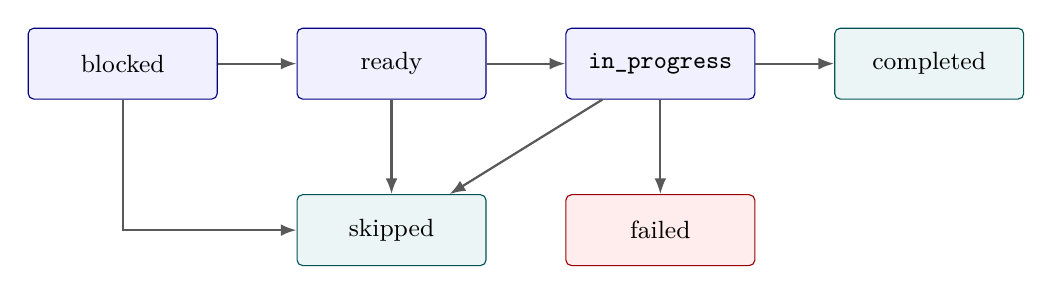
\begin{tikzpicture}[
  font=\small,
  state/.style={draw=blue!50!black, rounded corners=2pt, fill=blue!6,
    minimum width=24mm, minimum height=9mm, align=center},
  terminal/.style={state, draw=teal!65!black, fill=teal!8},
  error/.style={state, draw=red!60!black, fill=red!7},
  flow/.style={-{Latex[length=2mm]}, thick, draw=black!65}
]
\node[state] (blocked) {blocked};
\node[state, right=10mm of blocked] (ready) {ready};
\node[state, right=10mm of ready] (progress) {\texttt{in\_progress}};
\node[terminal, right=10mm of progress] (completed) {completed};
\node[terminal, below=12mm of ready] (skipped) {skipped};
\node[error, below=12mm of progress] (failed) {failed};

\draw[flow] (blocked) -- (ready);
\draw[flow] (ready) -- (progress);
\draw[flow] (progress) -- (completed);
\draw[flow] (blocked) |- (skipped);
\draw[flow] (ready) -- (skipped);
\draw[flow] (progress) -- (skipped);
\draw[flow] (progress) -- (failed);
\end{tikzpicture}
\caption{Work-item states are identical for human- and LLM-performed work.
Completed, skipped, and failed are terminal.}
\label{fig:work-item-lifecycle}
\end{figure}

\begin{description}
\tightlist
\item[\texttt{blocked}]
The dependencies have not reached terminal states.
\item[\texttt{ready}]
Dependencies are terminal and the enable condition is true. A durable
outbox record exists for delivery.
\item[\texttt{in\_progress}]
The survey was opened or an execution attempt acquired a lease.
\item[\texttt{completed}]
A valid answer was submitted exactly once.
\item[\texttt{skipped}]
A dependency was skipped, a condition evaluated false, quorum superseded
the assignment, or a repeat terminated before this iteration.
\item[\texttt{failed}]
The configured retry budget was exhausted or an error was classified as
non-retryable.
\end{description}

A dependency is settled when all of its work items are
\texttt{completed} or \texttt{skipped}. A failed item instead fails its
workflow instance.

\chapter{Participant selection and
fan-out}\label{participant-selection-and-fan-out}

\texttt{role(name)} constructs an exact trait selector:

\begin{Shaded}
\begin{Highlighting}[]
\NormalTok{review }\OperatorTok{=}\NormalTok{ builder.step(}
    \StringTok{"review"}\NormalTok{,}
\NormalTok{    review\_survey,}
\NormalTok{    assigned\_to}\OperatorTok{=}\NormalTok{role(}\StringTok{"reviewer"}\NormalTok{),}
\NormalTok{)}
\end{Highlighting}
\end{Shaded}

Every participant with \texttt{traits{[}"role"{]}\ ==\ "reviewer"}
receives an independent work item. This is fan-out.

The underlying selector can match several traits:

\begin{Shaded}
\begin{Highlighting}[]
\ImportTok{from}\NormalTok{ edsl.workflows }\ImportTok{import}\NormalTok{ ParticipantSelector}

\NormalTok{senior\_economists }\OperatorTok{=}\NormalTok{ ParticipantSelector(}
\NormalTok{    \{}\StringTok{"role"}\NormalTok{: }\StringTok{"reviewer"}\NormalTok{, }\StringTok{"discipline"}\NormalTok{: }\StringTok{"economics"}\NormalTok{, }\StringTok{"seniority"}\NormalTok{: }\StringTok{"senior"}\NormalTok{\}}
\NormalTok{)}
\end{Highlighting}
\end{Shaded}

Matching is exact and conjunctive. There is not yet an expression
language for inequalities, membership, or arbitrary roster queries.

Every step must match at least one participant at launch. Duplicate
participant names are rejected because the name is the durable
participant identifier.

\chapter{Dependencies and fan-in}\label{dependencies-and-fan-in}

Pass a step handle through \texttt{after}:

\begin{Shaded}
\begin{Highlighting}[]
\NormalTok{draft }\OperatorTok{=}\NormalTok{ builder.step(}\StringTok{"draft"}\NormalTok{, draft\_survey, assigned\_to}\OperatorTok{=}\NormalTok{role(}\StringTok{"author"}\NormalTok{))}
\NormalTok{review }\OperatorTok{=}\NormalTok{ builder.step(}
    \StringTok{"review"}\NormalTok{,}
\NormalTok{    review\_survey,}
\NormalTok{    assigned\_to}\OperatorTok{=}\NormalTok{role(}\StringTok{"reviewer"}\NormalTok{),}
\NormalTok{    after}\OperatorTok{=}\NormalTok{draft,}
\NormalTok{)}
\end{Highlighting}
\end{Shaded}

Multiple prerequisites form an AND dependency:

\begin{Shaded}
\begin{Highlighting}[]
\NormalTok{builder.step(}
    \StringTok{"release"}\NormalTok{,}
\NormalTok{    release\_survey,}
\NormalTok{    assigned\_to}\OperatorTok{=}\NormalTok{role(}\StringTok{"publisher"}\NormalTok{),}
\NormalTok{    after}\OperatorTok{=}\NormalTok{(legal\_review, technical\_review),}
\NormalTok{)}
\end{Highlighting}
\end{Shaded}

When a dependency has many assigned participants, the dependent step
waits for the dependency's completion policy. The default is all
assigned participants. This produces fan-in without a separate join
node.

Conditions automatically add the steps they reference to \texttt{after}.
Explicit \texttt{after} declarations are still recommended when they
explain the graph.

\chapter{Typed references}\label{typed-references}

Typed references reduce fragile, handwritten Jinja paths.

\section{One answer}\label{one-answer}

Use \texttt{answer()} when a source step has one relevant submission:

\begin{Shaded}
\begin{Highlighting}[]
\NormalTok{draft.answer(}\StringTok{"copy"}\NormalTok{).template}
\end{Highlighting}
\end{Shaded}

This renders a path under \texttt{workflow.answers}.

\section{All answers from a fan-out
step}\label{all-answers-from-a-fan-out-step}

Use \texttt{outputs()} when every submission matters:

\begin{Shaded}
\begin{Highlighting}[]
\NormalTok{reviews.outputs(}\StringTok{"decision"}\NormalTok{).template}
\end{Highlighting}
\end{Shaded}

This renders a list of values under \texttt{workflow.outputs}.

\section{Identity-preserving
submissions}\label{identity-preserving-submissions}

Some mechanisms need both identity and answers:

\begin{Shaded}
\begin{Highlighting}[]
\NormalTok{reports.submissions.template}
\end{Highlighting}
\end{Shaded}

The rendered structure is conceptually:

\begin{Shaded}
\begin{Highlighting}[]
\NormalTok{[}
\NormalTok{    \{}
        \StringTok{"participant\_id"}\NormalTok{: }\StringTok{"respondent{-}1"}\NormalTok{,}
        \StringTok{"answers"}\NormalTok{: \{}\StringTok{"signal"}\NormalTok{: }\StringTok{"Red"}\NormalTok{, }\StringTok{"forecast"}\NormalTok{: }\DecValTok{60}\NormalTok{\},}
\NormalTok{    \},}
    \CommentTok{\# ...}
\NormalTok{]}
\end{Highlighting}
\end{Shaded}

Use this only when identity is genuinely required. Anonymous synthesis
should usually consume \texttt{outputs()} instead.

\section{Fallback references}\label{fallback-references}

A branch may produce either an original or revised artifact:

\begin{Shaded}
\begin{Highlighting}[]
\NormalTok{latest }\OperatorTok{=}\NormalTok{ revision.answer(}\StringTok{"copy"}\NormalTok{).template\_or(draft.answer(}\StringTok{"copy"}\NormalTok{))}
\end{Highlighting}
\end{Shaded}

The fallback is evaluated during survey rendering. It does not execute
Python at workflow runtime.

\chapter{Conditions and branching}\label{conditions-and-branching}

Conditions are serializable predicates. A step runs only when its
\texttt{when} condition evaluates true after all condition dependencies
settle.

\section{Answer equality}\label{answer-equality}

\begin{Shaded}
\begin{Highlighting}[]
\NormalTok{approved }\OperatorTok{=}\NormalTok{ review.answer(}\StringTok{"approved"}\NormalTok{).equals(}\StringTok{"Yes"}\NormalTok{)}

\NormalTok{builder.step(}\StringTok{"publish"}\NormalTok{, ..., when}\OperatorTok{=}\NormalTok{approved)}
\NormalTok{builder.step(}\StringTok{"revise"}\NormalTok{, ..., when}\OperatorTok{=}\NormalTok{not\_(approved))}
\end{Highlighting}
\end{Shaded}

\texttt{if\_(condition)} returns complementary \texttt{then} and
\texttt{otherwise} conditions:

\begin{Shaded}
\begin{Highlighting}[]
\NormalTok{branch }\OperatorTok{=}\NormalTok{ if\_(approved)}
\NormalTok{builder.step(}\StringTok{"publish"}\NormalTok{, ..., when}\OperatorTok{=}\NormalTok{branch.then)}
\NormalTok{builder.step(}\StringTok{"revise"}\NormalTok{, ..., when}\OperatorTok{=}\NormalTok{branch.otherwise)}
\end{Highlighting}
\end{Shaded}

\section{Boolean composition}\label{boolean-composition}

\begin{Shaded}
\begin{Highlighting}[]
\NormalTok{all\_of(legal\_ok, technical\_ok)}
\NormalTok{any\_of(editorial\_ok, emergency\_override)}
\NormalTok{not\_(rejected)}
\NormalTok{join\_all(a, b)}
\NormalTok{join\_any(a, b)}
\end{Highlighting}
\end{Shaded}

\texttt{all\_of} and \texttt{any\_of} require at least one argument.

\section{Aggregate predicates}\label{aggregate-predicates}

\begin{Shaded}
\begin{Highlighting}[]
\NormalTok{votes.outputs(}\StringTok{"choice"}\NormalTok{).count(}\StringTok{"Approve"}\NormalTok{).at\_least(}\DecValTok{2}\NormalTok{)}
\NormalTok{votes.outputs(}\StringTok{"choice"}\NormalTok{).has\_disagreement}
\NormalTok{votes.outputs(}\StringTok{"choice"}\NormalTok{).majority\_is(}\StringTok{"Approve"}\NormalTok{)}
\NormalTok{estimates.outputs(}\StringTok{"value"}\NormalTok{).range\_at\_most(}\DecValTok{10}\NormalTok{)}
\end{Highlighting}
\end{Shaded}

\section{Stable chance}\label{stable-chance}

\begin{Shaded}
\begin{Highlighting}[]
\NormalTok{chance(}\FloatTok{0.70}\NormalTok{, key}\OperatorTok{=}\StringTok{"continue{-}after{-}round{-}2"}\NormalTok{)}
\end{Highlighting}
\end{Shaded}

Chance is deterministic for one \texttt{(instance\_id,\ key)} pair.
Reevaluation and process restart therefore cannot change the draw.
Always choose a stable, meaningful key.

\chapter{Completion policies and
quorum}\label{completion-policies-and-quorum}

The default completion policy is \texttt{all\_assigned()}.

For early fan-in, use quorum:

\begin{Shaded}
\begin{Highlighting}[]
\NormalTok{votes }\OperatorTok{=}\NormalTok{ builder.step(}
    \StringTok{"moderator{-}vote"}\NormalTok{,}
\NormalTok{    vote\_survey,}
\NormalTok{    assigned\_to}\OperatorTok{=}\NormalTok{role(}\StringTok{"moderator"}\NormalTok{),}
\NormalTok{    completion}\OperatorTok{=}\NormalTok{quorum(}\DecValTok{2}\NormalTok{),}
\NormalTok{)}
\end{Highlighting}
\end{Shaded}

Once two submissions complete, remaining work items for that step are
skipped as superseded. Downstream work may then proceed. A quorum larger
than the number of matching participants is rejected during launch.

Quorum does not presently express weighted votes, role-specific quotas,
or deadline-based partial completion.

\chapter{Deterministic derived
values}\label{deterministic-derived-values}

Language models should interpret evidence, not perform authoritative
arithmetic. Derived values provide a serializable calculation layer
modeled on the shared-state expression DSL.

\begin{Shaded}
\begin{Highlighting}[]
\NormalTok{stats }\OperatorTok{=}\NormalTok{ builder.derive(}
    \StringTok{"round{-}2{-}statistics"}\NormalTok{,}
\NormalTok{    mean}\OperatorTok{=}\NormalTok{round\_2.outputs(}\StringTok{"estimate"}\NormalTok{).mean(),}
\NormalTok{    median}\OperatorTok{=}\NormalTok{round\_2.outputs(}\StringTok{"estimate"}\NormalTok{).median(),}
\NormalTok{    minimum}\OperatorTok{=}\NormalTok{round\_2.outputs(}\StringTok{"estimate"}\NormalTok{).minimum(),}
\NormalTok{    maximum}\OperatorTok{=}\NormalTok{round\_2.outputs(}\StringTok{"estimate"}\NormalTok{).maximum(),}
\NormalTok{    spread}\OperatorTok{=}\NormalTok{round\_2.outputs(}\StringTok{"estimate"}\NormalTok{).}\BuiltInTok{range}\NormalTok{(),}
\NormalTok{)}
\end{Highlighting}
\end{Shaded}

Reference a field in a prompt:

\begin{Shaded}
\begin{Highlighting}[]
\NormalTok{QuestionFreeText(}
\NormalTok{    question\_name}\OperatorTok{=}\StringTok{"summary"}\NormalTok{,}
\NormalTok{    question\_text}\OperatorTok{=}\NormalTok{(}
        \SpecialStringTok{f"The authoritative mean is }\SpecialCharTok{\{}\NormalTok{stats}\SpecialCharTok{.}\NormalTok{field(}\StringTok{\textquotesingle{}mean\textquotesingle{}}\NormalTok{)}\SpecialCharTok{.}\NormalTok{template}\SpecialCharTok{\}}\SpecialStringTok{; "}
        \SpecialStringTok{f"the range is }\SpecialCharTok{\{}\NormalTok{stats}\SpecialCharTok{.}\NormalTok{field(}\StringTok{\textquotesingle{}spread\textquotesingle{}}\NormalTok{)}\SpecialCharTok{.}\NormalTok{template}\SpecialCharTok{\}}\SpecialStringTok{. Interpret them."}
\NormalTok{    ),}
\NormalTok{)}
\end{Highlighting}
\end{Shaded}

Or use a derived field in a condition:

\begin{Shaded}
\begin{Highlighting}[]
\NormalTok{converged }\OperatorTok{=}\NormalTok{ stats.field(}\StringTok{"spread"}\NormalTok{).at\_most(}\DecValTok{10}\NormalTok{)}
\end{Highlighting}
\end{Shaded}

Derived fields may reference earlier derived fields:

\begin{Shaded}
\begin{Highlighting}[]
\NormalTok{outcome }\OperatorTok{=}\NormalTok{ builder.derive(}
    \StringTok{"round{-}2{-}outcome"}\NormalTok{,}
\NormalTok{    converged}\OperatorTok{=}\NormalTok{stats.field(}\StringTok{"spread"}\NormalTok{).expression.compare\_at\_most(}\DecValTok{10}\NormalTok{),}
\NormalTok{)}
\end{Highlighting}
\end{Shaded}

The resulting expression tree contains named, allowlisted operators. It
has no callable, module path, source code, \texttt{eval}, or lambda.
This is invalid:

\begin{Shaded}
\begin{Highlighting}[]
\NormalTok{builder.derive(}\StringTok{"unsafe"}\NormalTok{, mean}\OperatorTok{=}\KeywordTok{lambda}\NormalTok{ values: }\BuiltInTok{sum}\NormalTok{(values) }\OperatorTok{/} \BuiltInTok{len}\NormalTok{(values))}
\end{Highlighting}
\end{Shaded}

The builder rejects it because derived fields must be
\texttt{WorkflowExpression} objects.

\section{Expression serialization}\label{expression-serialization}

A mean expression resembles:

\begin{Shaded}
\begin{Highlighting}[]
\FunctionTok{\{}
  \DataTypeTok{"type"}\FunctionTok{:} \StringTok{"workflow\_expression"}\FunctionTok{,}
  \DataTypeTok{"op"}\FunctionTok{:} \StringTok{"mean"}\FunctionTok{,}
  \DataTypeTok{"args"}\FunctionTok{:} \OtherTok{[}
    \FunctionTok{\{}
      \DataTypeTok{"type"}\FunctionTok{:} \StringTok{"workflow\_expression"}\FunctionTok{,}
      \DataTypeTok{"op"}\FunctionTok{:} \StringTok{"step\_outputs"}\FunctionTok{,}
      \DataTypeTok{"options"}\FunctionTok{:} \FunctionTok{\{}
        \DataTypeTok{"step\_name"}\FunctionTok{:} \StringTok{"round{-}2"}\FunctionTok{,}
        \DataTypeTok{"question\_name"}\FunctionTok{:} \StringTok{"estimate"}
      \FunctionTok{\}}
    \FunctionTok{\}}
  \OtherTok{]}\FunctionTok{,}
  \DataTypeTok{"options"}\FunctionTok{:} \FunctionTok{\{\}}
\FunctionTok{\}}
\end{Highlighting}
\end{Shaded}

Deserialization rejects unknown operators. Dependencies are extracted
from the tree and checked against the workflow. Derived references must
name an earlier definition and an existing field.

\section{Supported expression
operations}\label{supported-expression-operations}

The current evaluator supports:

\begin{Shaded}
\begin{Highlighting}[]
\NormalTok{Sources:      step\_outputs, derived\_ref}
\NormalTok{Aggregates:   mean, median, minimum, maximum, range}
\NormalTok{Arithmetic:   add, subtract, multiply, divide}
\NormalTok{Comparisons:  at\_most, at\_least, equals}
\end{Highlighting}
\end{Shaded}

Missing source outputs delay availability. Non-numeric values cause
numeric aggregates to fail rather than silently inventing coercions
beyond \texttt{float()}.

\chapter{Economic settlement
primitives}\label{economic-settlement-primitives}

Workflow expressions can consume a single answer or identity-preserving
submissions. This supports authoritative arithmetic without asking a
model to calculate payoffs:

\begin{Shaded}
\begin{Highlighting}[]
\NormalTok{accepted }\OperatorTok{=}\NormalTok{ response.answer(}\StringTok{"accept"}\NormalTok{).value.compare\_equals(}\StringTok{"Yes"}\NormalTok{)}
\NormalTok{payoffs }\OperatorTok{=}\NormalTok{ builder.derive(}
    \StringTok{"payoffs"}\NormalTok{,}
\NormalTok{    proposer}\OperatorTok{=}\NormalTok{choose(accepted, }\DecValTok{10} \OperatorTok{{-}}\NormalTok{ offer.answer(}\StringTok{"offer"}\NormalTok{).value, }\DecValTok{0}\NormalTok{),}
\NormalTok{    responder}\OperatorTok{=}\NormalTok{choose(accepted, offer.answer(}\StringTok{"offer"}\NormalTok{).value, }\DecValTok{0}\NormalTok{),}
\NormalTok{)}
\end{Highlighting}
\end{Shaded}

Two-player normal-form games use a serializable payoff matrix. Explicit
action codes avoid ambiguity when labels share an initial letter; matrix
keys concatenate the codes in stable participant-ID order:

\begin{Shaded}
\begin{Highlighting}[]
\NormalTok{payoffs }\OperatorTok{=}\NormalTok{ choices.submissions.payoff\_matrix(}
    \StringTok{"action"}\NormalTok{,}
\NormalTok{    \{}\StringTok{"WW"}\NormalTok{: (}\DecValTok{2}\NormalTok{, }\DecValTok{2}\NormalTok{), }\StringTok{"WT"}\NormalTok{: (}\DecValTok{1}\NormalTok{, }\DecValTok{3}\NormalTok{), }\StringTok{"TW"}\NormalTok{: (}\DecValTok{3}\NormalTok{, }\DecValTok{1}\NormalTok{), }\StringTok{"TT"}\NormalTok{: (}\DecValTok{0}\NormalTok{, }\DecValTok{0}\NormalTok{)\},}
\NormalTok{    action\_codes}\OperatorTok{=}\NormalTok{\{}\StringTok{"Swerve"}\NormalTok{: }\StringTok{"W"}\NormalTok{, }\StringTok{"Straight"}\NormalTok{: }\StringTok{"T"}\NormalTok{\},}
\NormalTok{)}
\end{Highlighting}
\end{Shaded}

Codes must be unique one-character strings. Omitting
\texttt{action\_codes} retains the legacy first-character convention for
serialized workflows created before this option was introduced.

\texttt{closest\_to(question,\ target,\ ties="all")} performs
identity-aware ranking. \texttt{DerivedFieldRef.for\_participant()}
projects an identity-keyed mapping into a private recipient prompt.
\texttt{match(role("player"),\ size=2)} deterministically partitions a
roster and round-trips as data.

Dynamic answer bounds are enforced when an answer is submitted:

\begin{Shaded}
\begin{Highlighting}[]
\NormalTok{builder.step(}
    \StringTok{"return"}\NormalTok{,}
\NormalTok{    return\_survey,}
\NormalTok{    after}\OperatorTok{=}\NormalTok{sent,}
\NormalTok{    answer\_bounds}\OperatorTok{=}\NormalTok{\{returned\_question: (}\DecValTok{0}\NormalTok{, sent.answer(}\StringTok{"sent"}\NormalTok{).value }\OperatorTok{*} \DecValTok{3}\NormalTok{)\},}
\NormalTok{)}
\end{Highlighting}
\end{Shaded}

Static survey bounds remain useful for presentation; dynamic bounds are
the coordinator's authoritative validation rule.

\chapter{Bounded repetition}\label{bounded-repetition}

Many workflows are conceptually loops: Delphi rounds, revision cycles,
negotiations, repeated games, and retry-until-accepted tasks.

Use a repeat block to avoid manually defining every round:

\begin{Shaded}
\begin{Highlighting}[]
\KeywordTok{def}\NormalTok{ build\_round(iteration):}
\NormalTok{    estimate }\OperatorTok{=}\NormalTok{ QuestionNumerical(}
\NormalTok{        question\_name}\OperatorTok{=}\StringTok{"estimate"}\NormalTok{,}
\NormalTok{        question\_text}\OperatorTok{=}\SpecialStringTok{f"Round }\SpecialCharTok{\{}\NormalTok{iteration}\SpecialCharTok{.}\NormalTok{number}\SpecialCharTok{\}}\SpecialStringTok{: give your estimate."}\NormalTok{,}
\NormalTok{        min\_value}\OperatorTok{=}\DecValTok{0}\NormalTok{,}
\NormalTok{        max\_value}\OperatorTok{=}\DecValTok{100}\NormalTok{,}
\NormalTok{    )}
\NormalTok{    forecast }\OperatorTok{=}\NormalTok{ iteration.step(}
        \StringTok{"round"}\NormalTok{,}
\NormalTok{        Survey([estimate]),}
\NormalTok{        assigned\_to}\OperatorTok{=}\NormalTok{role(}\StringTok{"expert"}\NormalTok{),}
\NormalTok{    )}
\NormalTok{    iteration.stop\_when(}
\NormalTok{        forecast.outputs(}\StringTok{"estimate"}\NormalTok{).}\BuiltInTok{range}\NormalTok{().at\_most(}\DecValTok{10}\NormalTok{)}
\NormalTok{    )}

\NormalTok{rounds }\OperatorTok{=}\NormalTok{ builder.repeat(}
    \StringTok{"delphi{-}rounds"}\NormalTok{,}
\NormalTok{    min\_iterations}\OperatorTok{=}\DecValTok{2}\NormalTok{,}
\NormalTok{    max\_iterations}\OperatorTok{=}\DecValTok{3}\NormalTok{,}
\NormalTok{    build}\OperatorTok{=}\NormalTok{build\_round,}
\NormalTok{)}
\end{Highlighting}
\end{Shaded}

The \texttt{build} callable is authoring sugar. It runs while
constructing the definition and is not serialized. The compiled
\texttt{HumanWorkflow} contains a \texttt{RepeatBlock} with bounds,
iteration numbers, materialized step names, typed stop conditions, and
repeat metadata on each step.

This distinction is important:

\begin{itemize}
\tightlist
\item
  bounded iterations are materialized during authoring;
\item
  the persisted definition contains only data;
\item
  execution after deserialization does not need \texttt{build\_round};
  and
\item
  future iterations are skipped when the prior stop condition succeeds.
\end{itemize}

\texttt{min\_iterations} forces early rounds to run even if their stop
conditions are already true. \texttt{max\_iterations} is a hard safety
bound.

The current implementation is not an unbounded runtime loop. Large or
data-dependent iteration counts will eventually require runtime
materialization of a serializable subworkflow template.

\chapter{Output visibility and
confidentiality}\label{output-visibility-and-confidentiality}

By default, a step's outputs are available to downstream assignees.
Restrict them with \texttt{visible\_to}:

\begin{Shaded}
\begin{Highlighting}[]
\NormalTok{sealed }\OperatorTok{=}\NormalTok{ builder.step(}
    \StringTok{"sealed{-}bid"}\NormalTok{,}
\NormalTok{    bid\_survey,}
\NormalTok{    assigned\_to}\OperatorTok{=}\NormalTok{role(}\StringTok{"vendor"}\NormalTok{),}
\NormalTok{    visible\_to}\OperatorTok{=}\NormalTok{role(}\StringTok{"buyer"}\NormalTok{),}
\NormalTok{)}
\end{Highlighting}
\end{Shaded}

Several roles may be authorized:

\begin{Shaded}
\begin{Highlighting}[]
\NormalTok{visible\_to}\OperatorTok{=}\NormalTok{(role(}\StringTok{"expert"}\NormalTok{), role(}\StringTok{"facilitator"}\NormalTok{))}
\end{Highlighting}
\end{Shaded}

During compilation, EDSL rejects a typed reference when the consumer's
selector can never satisfy the source visibility policy. Visibility also
propagates through derived values: computing a mean from sealed bids
does not make that mean public automatically.

This is a definition-level information-flow check, not a complete
security system. Operational deployments must also secure SQLite files,
application logs, email content, Humanize access, credentials, and
administrator tooling.

An explicit anonymity policy with pseudonyms and identity audit rules
remains a future extension. Today, anonymous synthesis is expressed by
sending answer values without \texttt{participant\_id} and limiting
source visibility.

\chapter{Shared state inside
workflows}\label{shared-state-inside-workflows}

Dependencies move information between steps. Shared state provides
durable, typed resources that several steps may read or update.

Two convenience resources are available:

\begin{Shaded}
\begin{Highlighting}[]
\ImportTok{from}\NormalTok{ edsl.workflows }\ImportTok{import}\NormalTok{ Artifact, Collection}

\NormalTok{submission }\OperatorTok{=}\NormalTok{ Artifact(}\StringTok{"paper{-}submission"}\NormalTok{)}
\NormalTok{reviews }\OperatorTok{=}\NormalTok{ Collection(}\StringTok{"paper{-}reviews"}\NormalTok{)}
\end{Highlighting}
\end{Shaded}

An artifact is a write-once text value. A collection is an append-only
sequence of actor/value records. Both are ordinary
\texttt{SharedStateMap} definitions.

A step declares its accesses:

\begin{Shaded}
\begin{Highlighting}[]
\NormalTok{paper }\OperatorTok{=}\NormalTok{ submission.by(}\StringTok{"paper{-}1"}\NormalTok{).artifact}
\NormalTok{review\_log }\OperatorTok{=}\NormalTok{ reviews.by(}\StringTok{"paper{-}1"}\NormalTok{).collection}

\NormalTok{builder.step(}
    \StringTok{"submit"}\NormalTok{,}
\NormalTok{    submission\_survey,}
\NormalTok{    assigned\_to}\OperatorTok{=}\NormalTok{role(}\StringTok{"author"}\NormalTok{),}
\NormalTok{    writes}\OperatorTok{=}\NormalTok{(paper.submit(value}\OperatorTok{=}\NormalTok{submission\_question.answer),),}
\NormalTok{)}

\NormalTok{builder.step(}
    \StringTok{"review"}\NormalTok{,}
\NormalTok{    review\_survey,}
\NormalTok{    assigned\_to}\OperatorTok{=}\NormalTok{role(}\StringTok{"reviewer"}\NormalTok{),}
\NormalTok{    after}\OperatorTok{=}\NormalTok{submit,}
\NormalTok{    reads}\OperatorTok{=}\NormalTok{(paper.read(),),}
\NormalTok{    writes}\OperatorTok{=}\NormalTok{(}
\NormalTok{        review\_log.add(}
\NormalTok{            actor}\OperatorTok{=}\NormalTok{current.agent.name,}
\NormalTok{            value}\OperatorTok{=}\NormalTok{review\_question.answer,}
\NormalTok{        ),}
\NormalTok{    ),}
\NormalTok{)}
\end{Highlighting}
\end{Shaded}

The coordinator renders reads into \texttt{shared\_state}, records the
observed state versions, applies writes after answer submission, and
rejects a submission if a shared-state command rejects its transition.

Shared-state semantics are documented in
\texttt{docs/shared\_state\_dsl\_manual.md} and the normative material
under \texttt{docs/shared\_state\_semantics/}.

\chapter{Persistence with SQLite}\label{persistence-with-sqlite}

Create a local durable store:

\begin{Shaded}
\begin{Highlighting}[]
\NormalTok{store }\OperatorTok{=}\NormalTok{ SQLiteWorkflowStore(}\StringTok{"runs/my{-}workflow/workflow.sqlite"}\NormalTok{)}
\end{Highlighting}
\end{Shaded}

The store maintains these logical records:

\begin{longtable}[]{@{}
  >{\raggedright\arraybackslash}p{(\linewidth - 2\tabcolsep) * \real{0.5000}}
  >{\raggedright\arraybackslash}p{(\linewidth - 2\tabcolsep) * \real{0.5000}}@{}}
\toprule\noalign{}
\begin{minipage}[b]{\linewidth}\raggedright
Record
\end{minipage} & \begin{minipage}[b]{\linewidth}\raggedright
Purpose
\end{minipage} \\
\midrule\noalign{}
\endhead
\bottomrule\noalign{}
\endlastfoot
\texttt{workflow\_instances} & Definition snapshot and overall status \\
\texttt{workflow\_participants} & Serialized EDSL agents \\
\texttt{workflow\_items} & Per-participant task lifecycle \\
\texttt{workflow\_submissions} & Idempotent answers \\
\texttt{workflow\_events} & Ordered audit history \\
\texttt{workflow\_outbox} & Durable delivery requests \\
\texttt{workflow\_external\_tasks} & Humanize/provider identifiers \\
\texttt{workflow\_item\_renders} & Exact rendered survey and state
snapshot \\
\texttt{workflow\_attempts} & Attempt number, lease, outcome, and error
class \\
\end{longtable}

The database is initialized additively. Opening an older workflow
database creates newly introduced tables without deleting existing
execution data.

\chapter{Opening and submitting work}\label{opening-and-submitting-work}

\texttt{coordinator.open(item\_id)}:

\begin{enumerate}
\def\labelenumi{\arabic{enumi}.}
\tightlist
\item
  verifies that the item is ready or in progress;
\item
  loads participant traits;
\item
  reads authorized shared state;
\item
  assembles prior visible answers and submissions;
\item
  evaluates available derived values;
\item
  renders every survey question;
\item
  saves the exact render and state versions; and
\item
  marks the item in progress.
\end{enumerate}

The returned \texttt{OpenedWorkItem} contains the rendered survey and
execution context.

Submit an answer with a stable idempotency key:

\begin{Shaded}
\begin{Highlighting}[]
\NormalTok{coordinator.submit(}
\NormalTok{    item\_id,}
\NormalTok{    \{}\StringTok{"approved"}\NormalTok{: }\StringTok{"Yes"}\NormalTok{\},}
\NormalTok{    idempotency\_key}\OperatorTok{=}\StringTok{"humanize:survey{-}response{-}uuid"}\NormalTok{,}
\NormalTok{)}
\end{Highlighting}
\end{Shaded}

Submitting the same key for the same item twice produces one durable
submission and one completion event. Reusing it for a different item is
not accepted as a valid completion.

\chapter{The durable outbox}\label{the-durable-outbox}

When an item becomes ready, the coordinator creates an outbox record in
the same workflow store. Delivery reads only pending records:

\begin{Shaded}
\begin{Highlighting}[]
\NormalTok{dispatcher }\OperatorTok{=}\NormalTok{ OutboxDispatcher(store, adapter)}
\NormalTok{receipts }\OperatorTok{=}\NormalTok{ dispatcher.dispatch()}
\end{Highlighting}
\end{Shaded}

Each \texttt{DeliveryRequest} contains:

\begin{Shaded}
\begin{Highlighting}[]
\NormalTok{idempotency\_key}
\NormalTok{instance\_id}
\NormalTok{work\_item\_id}
\NormalTok{step\_name}
\NormalTok{participant\_id}
\end{Highlighting}
\end{Shaded}

An adapter must use the idempotency key when its external system
supports one. The outbox protects the ready decision from a process
failure between graph evaluation and delivery.

The current dispatcher marks delivery after the adapter returns.
Production adapters must themselves be idempotent because a crash after
external delivery but before the local mark can cause redelivery.

\chapter{Humanize and real
respondents}\label{humanize-and-real-respondents}

\texttt{HumanizeDeliveryAdapter} is intentionally thin. For each ready
item it:

\begin{enumerate}
\def\labelenumi{\arabic{enumi}.}
\tightlist
\item
  opens and renders the participant-specific survey;
\item
  creates a private Humanize survey;
\item
  creates a delivery;
\item
  records the external survey and delivery identifiers; and
\item
  returns a delivery receipt.
\end{enumerate}

\begin{Shaded}
\begin{Highlighting}[]
\NormalTok{adapter }\OperatorTok{=}\NormalTok{ HumanizeDeliveryAdapter(}
\NormalTok{    coordinator,}
\NormalTok{    subject\_prefix}\OperatorTok{=}\StringTok{"Weekend activity"}\NormalTok{,}
\NormalTok{)}
\NormalTok{OutboxDispatcher(store, adapter).dispatch()}
\end{Highlighting}
\end{Shaded}

Later, polling imports completed responses:

\begin{Shaded}
\begin{Highlighting}[]
\NormalTok{completed\_count }\OperatorTok{=}\NormalTok{ adapter.poll\_completed()}
\end{Highlighting}
\end{Shaded}

For each response, the adapter calls \texttt{coordinator.submit()}. That
submission may make new items ready, after which the outbox dispatcher
delivers the next wave.

Humanize owns survey presentation, invitations, and response collection.
It does not need to understand the dependency graph.

\chapter{Simulated respondents}\label{simulated-respondents}

The simulation uses the same coordinator and store with an in-memory
inbox:

\begin{Shaded}
\begin{Highlighting}[]
\ImportTok{from}\NormalTok{ edsl }\ImportTok{import}\NormalTok{ Model}
\ImportTok{from}\NormalTok{ edsl.workflows }\ImportTok{import}\NormalTok{ EDSLAgentAnswerer, WorkflowSimulation}

\NormalTok{answerer }\OperatorTok{=}\NormalTok{ EDSLAgentAnswerer(}
\NormalTok{    Model(}\StringTok{"gpt{-}4o{-}mini"}\NormalTok{, service\_name}\OperatorTok{=}\StringTok{"openai"}\NormalTok{),}
\NormalTok{    run\_options}\OperatorTok{=}\NormalTok{\{}\StringTok{"disable\_remote\_inference"}\NormalTok{: }\VariableTok{False}\NormalTok{\},}
\NormalTok{)}

\NormalTok{simulation }\OperatorTok{=}\NormalTok{ WorkflowSimulation(}
\NormalTok{    coordinator,}
\NormalTok{    \{agent.name: agent }\ControlFlowTok{for}\NormalTok{ agent }\KeywordTok{in}\NormalTok{ participants\},}
\NormalTok{    answerer,}
\NormalTok{)}
\NormalTok{simulation.run(instance\_id)}
\end{Highlighting}
\end{Shaded}

\texttt{EDSLAgentAnswerer} runs each rendered survey through the
ordinary EDSL agent/model pipeline. A scripted object implementing
\texttt{answer(agent,\ opened)} is often better for deterministic tests.

\texttt{response\_delay} and the virtual clock can model elapsed time
without sleeping:

\begin{Shaded}
\begin{Highlighting}[]
\NormalTok{simulation }\OperatorTok{=}\NormalTok{ WorkflowSimulation(}
\NormalTok{    coordinator,}
\NormalTok{    agents,}
\NormalTok{    answerer,}
\NormalTok{    response\_delay}\OperatorTok{=}\NormalTok{timedelta(hours}\OperatorTok{=}\DecValTok{2}\NormalTok{),}
\NormalTok{)}
\end{Highlighting}
\end{Shaded}

\chapter{Durable attempts and
recovery}\label{durable-attempts-and-recovery}

Remote inference and external delivery fail in several distinguishable
places: submission, model execution, result retrieval, process shutdown,
and network timeout. A durable workflow must resume rather than restart
completed work.

Configure simulation recovery with \texttt{RetryPolicy}:

\begin{Shaded}
\begin{Highlighting}[]
\ImportTok{from}\NormalTok{ edsl.workflows }\ImportTok{import}\NormalTok{ RetryPolicy}

\NormalTok{simulation.run(}
\NormalTok{    instance\_id,}
\NormalTok{    resume}\OperatorTok{=}\VariableTok{True}\NormalTok{,}
\NormalTok{    retry\_policy}\OperatorTok{=}\NormalTok{RetryPolicy(}
\NormalTok{        max\_attempts}\OperatorTok{=}\DecValTok{3}\NormalTok{,}
\NormalTok{        lease\_seconds}\OperatorTok{=}\DecValTok{300}\NormalTok{,}
\NormalTok{        retryable}\OperatorTok{=}\NormalTok{(}\StringTok{"remote\_error"}\NormalTok{, }\StringTok{"timeout"}\NormalTok{, }\StringTok{"exception"}\NormalTok{),}
\NormalTok{    ),}
\NormalTok{)}
\end{Highlighting}
\end{Shaded}

\section{Attempt lifecycle}\label{attempt-lifecycle}

Before an answerer runs, the store creates a numbered attempt with a
lease:

\begin{figure}[htbp]
\centering
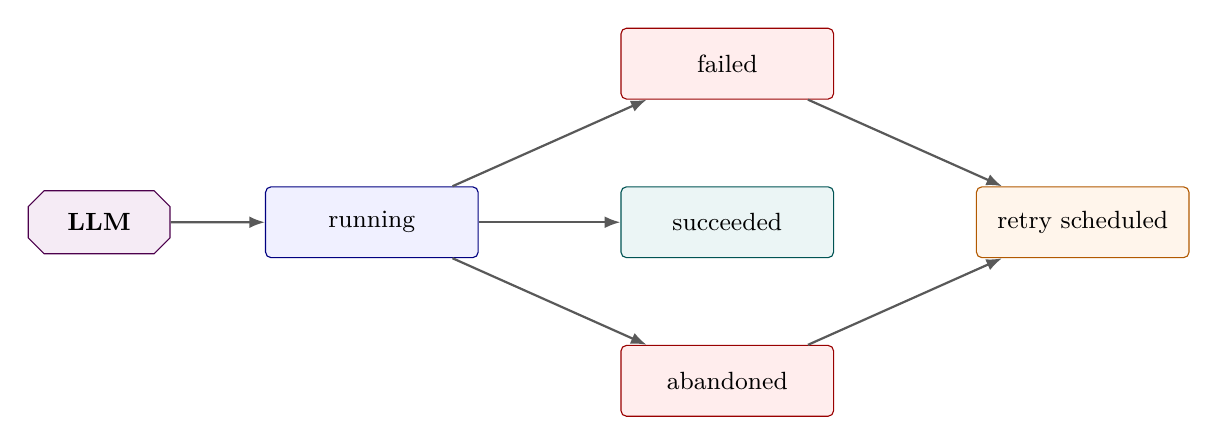
\begin{tikzpicture}[
  font=\small,
  state/.style={draw=blue!50!black, rounded corners=2pt, fill=blue!6,
    minimum width=27mm, minimum height=9mm, align=center},
  success/.style={state, draw=teal!65!black, fill=teal!8},
  error/.style={state, draw=red!60!black, fill=red!7},
  retry/.style={state, draw=orange!70!black, fill=orange!8},
  llm/.style={draw=violet!60!black, chamfered rectangle, chamfered rectangle corners=all,
    fill=violet!8, align=center, minimum width=18mm, minimum height=8mm},
  flow/.style={-{Latex[length=2mm]}, thick, draw=black!65}
]
\node[state] (running) {running};
\node[llm, left=12mm of running] (actor) {\textbf{LLM}};
\node[success, right=18mm of running] (succeeded) {succeeded};
\node[error, above=11mm of succeeded] (failed) {failed};
\node[error, below=11mm of succeeded] (abandoned) {abandoned};
\node[retry, right=18mm of succeeded] (retry) {retry scheduled};

\draw[flow] (actor) -- (running);
\draw[flow] (running) -- (succeeded);
\draw[flow] (running) -- (failed);
\draw[flow] (running) -- (abandoned);
\draw[flow] (failed) -- (retry);
\draw[flow] (abandoned) -- (retry);
\end{tikzpicture}
\caption{During LLM simulation, a durable answerer attempt either succeeds or
records why another attempt may be scheduled. Human delivery has its own
durable outbox and external-delivery records.}
\label{fig:attempt-lifecycle}
\end{figure}

Every attempt records its start, lease expiration, finish, status, error
kind, and a bounded error message.

\section{Leases}\label{leases}

A lease prevents two healthy workers from claiming the same in-progress
item. If the process disappears, another process can reclaim the item
after the lease expires. Recovery marks the old attempt
\texttt{abandoned} with \texttt{error\_kind="lease\_expired"} before
scheduling the next attempt.

Choose a lease comfortably longer than ordinary answer latency.
Automatic lease heartbeats are not yet implemented.

\section{Error classification}\label{error-classification}

The simulator currently classifies:

\begin{description}
\tightlist
\item[\texttt{timeout}]
Python \texttt{TimeoutError}.
\item[\texttt{remote\_error}]
Exception type identities containing \texttt{remote} or \texttt{coop}.
\item[\texttt{exception}]
Other exceptions.
\end{description}

Only listed classes are retried. Classification is intentionally
conservative and should eventually become a typed exception protocol
rather than a naming heuristic.

\section{Retry exhaustion}\label{retry-exhaustion}

After \texttt{max\_attempts}, the item becomes \texttt{failed} and the
workflow instance becomes \texttt{failed}. The simulator raises a
\texttt{RuntimeError} naming the failed steps. Failed instances do not
silently masquerade as completed runs.

\section{Restarting in a fresh
process}\label{restarting-in-a-fresh-process}

Reconstruct the definition and coordinator, then resume against the same
file:

\begin{Shaded}
\begin{Highlighting}[]
\NormalTok{restored }\OperatorTok{=}\NormalTok{ HumanWorkflow.from\_dict(saved\_definition)}
\NormalTok{store }\OperatorTok{=}\NormalTok{ SQLiteWorkflowStore(}\StringTok{"workflow.sqlite"}\NormalTok{)}
\NormalTok{coordinator }\OperatorTok{=}\NormalTok{ WorkflowCoordinator(restored, store)}
\NormalTok{simulation }\OperatorTok{=}\NormalTok{ WorkflowSimulation(coordinator, agents, answerer)}
\NormalTok{simulation.run(instance\_id, resume}\OperatorTok{=}\VariableTok{True}\NormalTok{, retry\_policy}\OperatorTok{=}\NormalTok{policy)}
\end{Highlighting}
\end{Shaded}

Recovery requeues:

\begin{itemize}
\tightlist
\item
  ready items whose earlier delivery record is no longer pending;
\item
  in-progress items with no active attempt; and
\item
  items whose running attempt lease expired.
\end{itemize}

It does not reclaim an item with an unexpired lease.

\chapter{Serialization and
portability}\label{serialization-and-portability}

Round-trip a workflow with:

\begin{Shaded}
\begin{Highlighting}[]
\NormalTok{payload }\OperatorTok{=}\NormalTok{ workflow.to\_dict()}
\NormalTok{restored }\OperatorTok{=}\NormalTok{ HumanWorkflow.from\_dict(payload)}
\ControlFlowTok{assert}\NormalTok{ restored.to\_dict() }\OperatorTok{==}\NormalTok{ payload}
\end{Highlighting}
\end{Shaded}

The serialized object includes:

\begin{Shaded}
\begin{Highlighting}[]
\FunctionTok{\{}
  \DataTypeTok{"type"}\FunctionTok{:} \StringTok{"human\_workflow"}\FunctionTok{,}
  \DataTypeTok{"version"}\FunctionTok{:} \DecValTok{1}\FunctionTok{,}
  \DataTypeTok{"name"}\FunctionTok{:} \StringTok{"Example"}\FunctionTok{,}
  \DataTypeTok{"steps"}\FunctionTok{:} \OtherTok{[]}\FunctionTok{,}
  \DataTypeTok{"metadata"}\FunctionTok{:} \FunctionTok{\{\},}
  \DataTypeTok{"derived\_values"}\FunctionTok{:} \OtherTok{[]}\FunctionTok{,}
  \DataTypeTok{"repeat\_blocks"}\FunctionTok{:} \OtherTok{[]}
\FunctionTok{\}}
\end{Highlighting}
\end{Shaded}

Surveys, selectors, conditions, completion policies, visibility
selectors, state reads and writes, derived expressions, and repeat
declarations all round-trip as data.

Execution policy such as a \texttt{RetryPolicy} is separately
serializable but is not currently embedded in \texttt{HumanWorkflow}.
This lets one deployment use a different operational retry budget
without changing the research design.

\chapter{Visualization and audit
evidence}\label{visualization-and-audit-evidence}

Render an instance as a standalone vertical DAG:

\begin{Shaded}
\begin{Highlighting}[]
\ImportTok{from}\NormalTok{ edsl.workflows }\ImportTok{import}\NormalTok{ WorkflowDAGVisualization}

\NormalTok{path }\OperatorTok{=}\NormalTok{ WorkflowDAGVisualization(coordinator, instance\_id).save(}\StringTok{"dag.html"}\NormalTok{)}
\end{Highlighting}
\end{Shaded}

The visualization shows:

\begin{itemize}
\tightlist
\item
  wall-clock ordering on the vertical axis;
\item
  dependency edges;
\item
  participant-specific colors;
\item
  question-type glyphs;
\item
  work-item status;
\item
  rendered question text and options;
\item
  submitted responses;
\item
  shared-state snapshots and transitions;
\item
  lifecycle timestamps;
\item
  execution attempts and error classifications; and
\item
  the ordered workflow event timeline.
\end{itemize}

Failed items are visually distinct. Repeat conditions and derived
expression conditions are rendered as readable labels.

The visualization reads persisted evidence. It does not rerun conditions
or call a model merely to construct the page.

\chapter{Pattern: parallel brainstorm and
selection}\label{pattern-parallel-brainstorm-and-selection}

\begin{Shaded}
\begin{Highlighting}[]
\NormalTok{ideas }\OperatorTok{=}\NormalTok{ builder.step(}
    \StringTok{"idea"}\NormalTok{,}
\NormalTok{    idea\_survey,}
\NormalTok{    assigned\_to}\OperatorTok{=}\NormalTok{role(}\StringTok{"ideator"}\NormalTok{),}
\NormalTok{)}

\NormalTok{builder.step(}
    \StringTok{"select"}\NormalTok{,}
\NormalTok{    Survey([}
\NormalTok{        QuestionFreeText(}
\NormalTok{            question\_name}\OperatorTok{=}\StringTok{"choice"}\NormalTok{,}
\NormalTok{            question\_text}\OperatorTok{=}\SpecialStringTok{f"Choose from }\SpecialCharTok{\{}\NormalTok{ideas}\SpecialCharTok{.}\NormalTok{outputs(}\StringTok{\textquotesingle{}idea\textquotesingle{}}\NormalTok{)}\SpecialCharTok{.}\NormalTok{template}\SpecialCharTok{\}}\SpecialStringTok{."}\NormalTok{,}
\NormalTok{        )}
\NormalTok{    ]),}
\NormalTok{    assigned\_to}\OperatorTok{=}\NormalTok{role(}\StringTok{"chair"}\NormalTok{),}
\NormalTok{    after}\OperatorTok{=}\NormalTok{ideas,}
\NormalTok{)}
\end{Highlighting}
\end{Shaded}

This is the simplest fan-out/fan-in pattern.

\chapter{Pattern: blind review}\label{pattern-blind-review}

An author writes an artifact. Several reviewers can read it but cannot
read one another's reviews. An editor receives the collected reviews.

Use output visibility for sealed responses and shared-state capabilities
for durable artifacts. Be explicit about which layer protects which
information.

\chapter{Pattern: approval with
revision}\label{pattern-approval-with-revision}

\begin{Shaded}
\begin{Highlighting}[]
\NormalTok{branch }\OperatorTok{=}\NormalTok{ if\_(review.answer(}\StringTok{"approved"}\NormalTok{).equals(}\StringTok{"Yes"}\NormalTok{))}

\NormalTok{revision }\OperatorTok{=}\NormalTok{ builder.step(}\StringTok{"revise"}\NormalTok{, ..., when}\OperatorTok{=}\NormalTok{branch.otherwise)}
\NormalTok{builder.step(}
    \StringTok{"publish"}\NormalTok{,}
\NormalTok{    Survey([}
\NormalTok{        QuestionFreeText(}
\NormalTok{            question\_name}\OperatorTok{=}\StringTok{"publication"}\NormalTok{,}
\NormalTok{            question\_text}\OperatorTok{=}\NormalTok{(}
                \StringTok{"Publish "}
                \SpecialStringTok{f"}\SpecialCharTok{\{}\NormalTok{revision}\SpecialCharTok{.}\NormalTok{answer(}\StringTok{\textquotesingle{}copy\textquotesingle{}}\NormalTok{)}\SpecialCharTok{.}\NormalTok{template\_or(draft.answer(}\StringTok{\textquotesingle{}copy\textquotesingle{}}\NormalTok{))}\SpecialCharTok{\}}\SpecialStringTok{"}
\NormalTok{            ),}
\NormalTok{        )}
\NormalTok{    ]),}
\NormalTok{    after}\OperatorTok{=}\NormalTok{(review, revision),}
\NormalTok{    when}\OperatorTok{=}\NormalTok{join\_any(branch.then, revision.completed),}
\NormalTok{)}
\end{Highlighting}
\end{Shaded}

This pattern demonstrates complementary branches and typed fallback
selection.

\chapter{Pattern: Delphi forecasting}\label{pattern-delphi-forecasting}

A Delphi workflow combines several features:

\begin{enumerate}
\def\labelenumi{\arabic{enumi}.}
\tightlist
\item
  experts answer independently;
\item
  only the facilitator sees identity-bearing source work;
\item
  the facilitator returns an anonymous synthesis;
\item
  derived expressions calculate authoritative statistics;
\item
  a bounded repeat continues for at least two rounds; and
\item
  a typed range condition stops later rounds after convergence.
\end{enumerate}

The simulation that motivated derived values revealed an important
principle: the facilitator correctly discussed disagreements but
misstated the arithmetic and termination result. The engine should
compute facts; the model should explain them.

\chapter{Pattern: probabilistically ending public-goods
game}\label{pattern-probabilistically-ending-public-goods-game}

\begin{Shaded}
\begin{Highlighting}[]
\KeywordTok{def}\NormalTok{ build\_round(iteration):}
\NormalTok{    previous }\OperatorTok{=}\NormalTok{ rounds\_by\_number.get(iteration.number }\OperatorTok{{-}} \DecValTok{1}\NormalTok{)}
    \CommentTok{\# Construct a survey referencing the previous contribution vector.}
\NormalTok{    current }\OperatorTok{=}\NormalTok{ iteration.step(}
        \StringTok{"round"}\NormalTok{,}
\NormalTok{        survey,}
\NormalTok{        assigned\_to}\OperatorTok{=}\NormalTok{role(}\StringTok{"player"}\NormalTok{),}
\NormalTok{    )}
\NormalTok{    iteration.stop\_when(}
\NormalTok{        not\_(chance(}\FloatTok{0.70}\NormalTok{, key}\OperatorTok{=}\SpecialStringTok{f"continue{-}after{-}round{-}}\SpecialCharTok{\{}\NormalTok{iteration}\SpecialCharTok{.}\NormalTok{number}\SpecialCharTok{\}}\SpecialStringTok{"}\NormalTok{))}
\NormalTok{    )}
\NormalTok{    rounds\_by\_number[iteration.number] }\OperatorTok{=}\NormalTok{ current}

\NormalTok{builder.repeat(}\StringTok{"public{-}goods{-}rounds"}\NormalTok{, max\_iterations}\OperatorTok{=}\DecValTok{5}\NormalTok{, build}\OperatorTok{=}\NormalTok{build\_round)}
\end{Highlighting}
\end{Shaded}

Stable chance ensures a restart cannot redraw whether the game
continues.

\chapter{Pattern: peer prediction}\label{pattern-peer-prediction}

Peer prediction requires identity-preserving sealed reports,
deterministic matching, and deterministic scoring. The current workflow
can deliver sealed submissions to a scorer, but scoring arithmetic
should be a derived expression or a future allowlisted algorithm---not
prose delegated to an LLM.

Per-recipient output projection is also important: respondents should
receive their own score rather than the full scoring table.

\chapter{Testing workflows}\label{testing-workflows}

Use scripted answerers for semantic tests:

\begin{Shaded}
\begin{Highlighting}[]
\KeywordTok{class}\NormalTok{ Answers:}
    \KeywordTok{def}\NormalTok{ answer(}\VariableTok{self}\NormalTok{, agent, opened):}
        \ControlFlowTok{if}\NormalTok{ opened.step\_name }\OperatorTok{==} \StringTok{"propose"}\NormalTok{:}
            \ControlFlowTok{return}\NormalTok{ \{}\StringTok{"activity"}\NormalTok{: }\StringTok{"Sailing"}\NormalTok{\}}
        \ControlFlowTok{return}\NormalTok{ \{}\StringTok{"approved"}\NormalTok{: }\StringTok{"Yes"}\NormalTok{\}}
\end{Highlighting}
\end{Shaded}

A strong workflow test should verify:

\begin{itemize}
\tightlist
\item
  definition serialization and reconstruction;
\item
  initial ready fan-out;
\item
  delivery order;
\item
  exact rendered downstream context;
\item
  completed and skipped work-item statuses;
\item
  condition decisions;
\item
  shared-state results and versions;
\item
  submission idempotency;
\item
  restart behavior using a new store and coordinator object;
\item
  retry exhaustion and workflow failure; and
\item
  visualization generation.
\end{itemize}

For derived expressions, also test rejection of raw Python and unknown
operators. For visibility, test that an unauthorized derived reference
fails compilation.

\chapter{Operational checklist}\label{operational-checklist}

Before a real deployment:

\begin{enumerate}
\def\labelenumi{\arabic{enumi}.}
\tightlist
\item
  Serialize and reconstruct the workflow in a fresh process.
\item
  Verify every role matches the intended participant count.
\item
  Audit every \texttt{visible\_to} declaration and identity-bearing
  submission.
\item
  Use stable idempotency keys in delivery and submission adapters.
\item
  Put the SQLite database on durable, access-controlled storage.
\item
  Choose lease durations longer than expected provider latency.
\item
  Restrict retryable errors and set a finite attempt budget.
\item
  Test a crash after delivery and a crash during answer retrieval.
\item
  Use deterministic expressions for arithmetic and authoritative
  decisions.
\item
  Render and inspect the DAG and event history.
\item
  Verify Humanize surveys are private where required.
\item
  Decide how operators are alerted when an instance fails.
\end{enumerate}

\chapter{Current limitations}\label{current-limitations}

The following are important but not yet first-class:

\begin{itemize}
\tightlist
\item
  runtime or unbounded repeat materialization;
\item
  lease heartbeat and active renewal;
\item
  a typed provider-error protocol;
\item
  automatic cancellation of external work after quorum or branch
  supersession;
\item
  deadlines, reminders, priorities, and escalation schedules;
\item
  explicit anonymous-panel and pseudonym policies;
\item
  per-recipient projection of a batch result;
\item
  persisted snapshots of every derived value and condition evaluation;
\item
  weighted quorum and richer participant selectors;
\item
  deterministic quantiles, variance, standard deviation, and frequency
  tables;
\item
  one \texttt{on\_termination} step for every possible repeat exit; and
\item
  transactional atomicity spanning workflow and separate shared-state
  databases.
\end{itemize}

These limitations are design boundaries, not invitations to hide
behavior in Python callbacks or LLM prompts. New capabilities should
extend the serializable DSL and coordinator evaluator.

\chapter{Compact API reference}\label{compact-api-reference}

\section{Authoring}\label{authoring}

\begin{Shaded}
\begin{Highlighting}[]
\NormalTok{Workflow(name, metadata}\OperatorTok{=}\VariableTok{None}\NormalTok{)}
\NormalTok{builder.step(name, survey, assigned\_to}\OperatorTok{=}\NormalTok{..., after}\OperatorTok{=}\NormalTok{..., when}\OperatorTok{=}\NormalTok{...,}
\NormalTok{             completion}\OperatorTok{=}\NormalTok{..., visible\_to}\OperatorTok{=}\NormalTok{..., reads}\OperatorTok{=}\NormalTok{..., writes}\OperatorTok{=}\NormalTok{..., metadata}\OperatorTok{=}\NormalTok{...)}
\NormalTok{builder.derive(name, }\OperatorTok{**}\NormalTok{workflow\_expressions)}
\NormalTok{builder.repeat(name, min\_iterations}\OperatorTok{=}\DecValTok{1}\NormalTok{, max\_iterations}\OperatorTok{=}\NormalTok{N,}
\NormalTok{               build}\OperatorTok{=}\NormalTok{authoring\_callback, after}\OperatorTok{=}\VariableTok{None}\NormalTok{)}
\NormalTok{builder.}\BuiltInTok{compile}\NormalTok{() }\OperatorTok{{-}\textgreater{}}\NormalTok{ HumanWorkflow}
\end{Highlighting}
\end{Shaded}

\section{Selectors and policies}\label{selectors-and-policies}

\begin{Shaded}
\begin{Highlighting}[]
\NormalTok{role(name)}
\NormalTok{ParticipantSelector(mapping)}
\NormalTok{all\_assigned()}
\NormalTok{quorum(count)}
\end{Highlighting}
\end{Shaded}

\section{Conditions}\label{conditions}

\begin{Shaded}
\begin{Highlighting}[]
\NormalTok{answer.equals(value)}
\NormalTok{step.completed}
\NormalTok{all\_of(}\OperatorTok{*}\NormalTok{conditions)}
\NormalTok{any\_of(}\OperatorTok{*}\NormalTok{conditions)}
\NormalTok{not\_(condition)}
\NormalTok{if\_(condition)}
\NormalTok{chance(probability, key}\OperatorTok{=}\NormalTok{stable\_key)}
\NormalTok{outputs.count(value).at\_least(count)}
\NormalTok{outputs.has\_disagreement}
\NormalTok{outputs.majority\_is(value)}
\NormalTok{outputs.range\_at\_most(maximum)}
\NormalTok{derived\_field.at\_most(value)}
\NormalTok{derived\_field.at\_least(value)}
\NormalTok{derived\_field.equals(value)}
\end{Highlighting}
\end{Shaded}

\section{Execution}\label{execution}

\begin{Shaded}
\begin{Highlighting}[]
\NormalTok{SQLiteWorkflowStore(path)}
\NormalTok{WorkflowCoordinator(workflow, store, state\_backends}\OperatorTok{=}\VariableTok{None}\NormalTok{)}
\NormalTok{coordinator.launch(participants, instance\_id}\OperatorTok{=}\VariableTok{None}\NormalTok{)}
\NormalTok{coordinator.}\BuiltInTok{open}\NormalTok{(work\_item\_id)}
\NormalTok{coordinator.submit(work\_item\_id, answers, idempotency\_key}\OperatorTok{=}\NormalTok{...)}
\NormalTok{OutboxDispatcher(store, adapter).dispatch()}
\NormalTok{WorkflowSimulation(coordinator, agents, answerer).run(}
\NormalTok{    instance\_id,}
\NormalTok{    resume}\OperatorTok{=}\VariableTok{False}\NormalTok{,}
\NormalTok{    retry\_policy}\OperatorTok{=}\NormalTok{RetryPolicy(),}
\NormalTok{)}
\end{Highlighting}
\end{Shaded}

\section{Inspection}\label{inspection}

\begin{Shaded}
\begin{Highlighting}[]
\NormalTok{store.items(instance\_id)}
\NormalTok{store.item\_answers(work\_item\_id)}
\NormalTok{store.step\_answers(instance\_id, step\_name)}
\NormalTok{store.events(instance\_id)}
\NormalTok{store.attempts(work\_item\_id)}
\NormalTok{WorkflowDAGVisualization(coordinator, instance\_id).save(path)}
\end{Highlighting}
\end{Shaded}

\chapter{Closing principle}\label{closing-principle}

A trustworthy workflow keeps four responsibilities separate:

\begin{figure}[htbp]
\centering
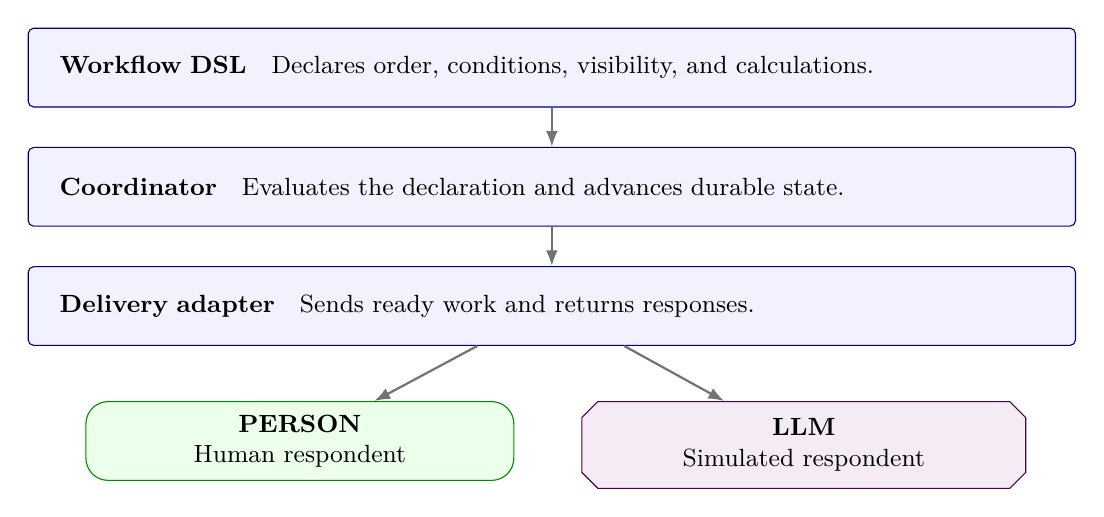
\begin{tikzpicture}[
  font=\small,
  layer/.style={draw=blue!50!black, rounded corners=2pt, fill=blue!5,
    minimum height=10mm, text width=125mm, align=left, inner xsep=4mm},
  human/.style={draw=green!55!black, rounded corners=8pt, fill=green!8,
    minimum height=10mm, text width=52mm, align=center},
  llm/.style={draw=violet!60!black, chamfered rectangle, chamfered rectangle corners=all,
    fill=violet!8, minimum height=10mm, text width=52mm, align=center},
  flow/.style={-{Latex[length=2mm]}, thick, draw=black!55}
]
\node[layer] (dsl) {\textbf{Workflow DSL}\quad Declares order, conditions,
visibility, and calculations.};
\node[layer, below=5mm of dsl] (coord) {\textbf{Coordinator}\quad Evaluates the
declaration and advances durable state.};
\node[layer, below=5mm of coord] (delivery) {\textbf{Delivery adapter}\quad Sends
ready work and returns responses.};
\node[human, below=7mm of delivery, xshift=-32mm] (person)
  {\textbf{PERSON}\\Human respondent};
\node[llm, below=7mm of delivery, xshift=32mm] (llm)
  {\textbf{LLM}\\Simulated respondent};
\draw[flow] (dsl) -- (coord);
\draw[flow] (coord) -- (delivery);
\draw[flow] (delivery) -- (person);
\draw[flow] (delivery) -- (llm);
\end{tikzpicture}
\caption{The responsibility boundaries in a workflow deployment. The delivery
path terminates in either a person or an LLM; the workflow definition itself is
the same.}
\label{fig:responsibility-boundaries}
\end{figure}

When arithmetic, routing, retries, or confidentiality matter, they
belong in the first two layers. Human and LLM respondents should receive
well-defined work, not responsibility for enforcing the protocol that
assigned it.

\chapter{Rebuilding this manual}\label{rebuilding-this-manual}

The Markdown source is converted to standalone LaTeX and then compiled
with XeLaTeX:

\begin{Shaded}
\begin{Highlighting}[]
\ExtensionTok{pandoc}\NormalTok{ docs/workflow\_manual.md }\DataTypeTok{\textbackslash{}}
  \AttributeTok{{-}{-}standalone} \AttributeTok{{-}{-}to}\OperatorTok{=}\NormalTok{latex }\DataTypeTok{\textbackslash{}}
  \AttributeTok{{-}{-}output}\OperatorTok{=}\NormalTok{docs/workflow\_manual.tex}

\ExtensionTok{xelatex} \AttributeTok{{-}interaction}\OperatorTok{=}\NormalTok{nonstopmode }\AttributeTok{{-}halt{-}on{-}error} \DataTypeTok{\textbackslash{}}
  \AttributeTok{{-}output{-}directory}\OperatorTok{=}\NormalTok{docs docs/workflow\_manual.tex}
\ExtensionTok{xelatex} \AttributeTok{{-}interaction}\OperatorTok{=}\NormalTok{nonstopmode }\AttributeTok{{-}halt{-}on{-}error} \DataTypeTok{\textbackslash{}}
  \AttributeTok{{-}output{-}directory}\OperatorTok{=}\NormalTok{docs docs/workflow\_manual.tex}
\end{Highlighting}
\end{Shaded}

The second XeLaTeX pass resolves the table of contents and page
references.

\end{document}
